\chapter{HANI Poroviscoelastic Characterization}\label{chap:5}

The Hybrid Hydrogels Augmented via Additive Network Integration (HANI) platform represents a novel approach to tissue engineering, specifically designed to address the complex mechanical requirements of meniscal tissue. By strategically integrating polycaprolactone (PCL) reinforcement networks within gelatin-based hydrogels, the HANI methodology creates composite scaffolds that combine the poroviscoelastic properties of hydrogels with the structural stability of thermoplastic reinforcement. While previous chapters have established the fabrication methodology, this chapter focuses on the comprehensive time-dependent mechanical characterization of these composite scaffolds.

Native meniscal tissue exhibits a unique set of mechanical properties that must be replicated by any viable replacement. These include appropriate stress response under compression, sustained load-bearing capacity, and viscoelastic behavior that facilitates energy dissipation during joint loading. The validation of static mechanical properties is therefore critical to assess whether HANI scaffolds can function effectively within the demanding mechanical environment of the knee joint.

The central research question addressed in this chapter examines whether PCL-reinforced gelatin hydrogels can replicate the peak and equilibrium stresses of native meniscal tissue under quasi-static loading conditions. Furthermore, this work investigates how variations in crosslinking density and PCL reinforcement architecture influence these mechanical parameters across physiologically relevant strain levels.

\section{Experimental Design and Methodology}

Two distinct gelatin-to-glutaraldehyde (GelA:GTA) mass ratios were selected for evaluation: 100:1 and 300:1. These formulations were chosen based on preliminary studies that demonstrated their capacity to maintain water content comparable to native meniscal tissue (approximately 76\%). The 100:1 ratio represents a higher crosslinking density expected to yield greater mechanical stiffness, while the 300:1 ratio provides a more compliant matrix with potentially enhanced fluid flow characteristics.

Four configurations were systematically evaluated to assess the impact of reinforcement architecture on mechanical performance:
\begin{itemize}
    \item \textbf{No PCL (Control)}: Hydrogel-only samples serving as baseline controls
    \item \textbf{Aligned PCL}: Linear PCL fibers with radial tie fibers for enhanced stability
    \item \textbf{Circumferential PCL}: Aligned fibers with additional circumferential bands to mimic the native meniscal collagen organization
    \item \textbf{3D PCL}: Thermomolded networks spanning the full hydrogel thickness to provide comprehensive three-dimensional reinforcement
\end{itemize}

This systematic approach to varying both crosslinking density and reinforcement architecture enables comprehensive evaluation of how these design parameters influence the mechanical properties of HANI scaffolds. By testing these configurations across multiple strain levels, we can identify optimal combinations that best replicate the complex mechanical behavior of native meniscal tissue.

\begin{figure}[H]
    \centering
    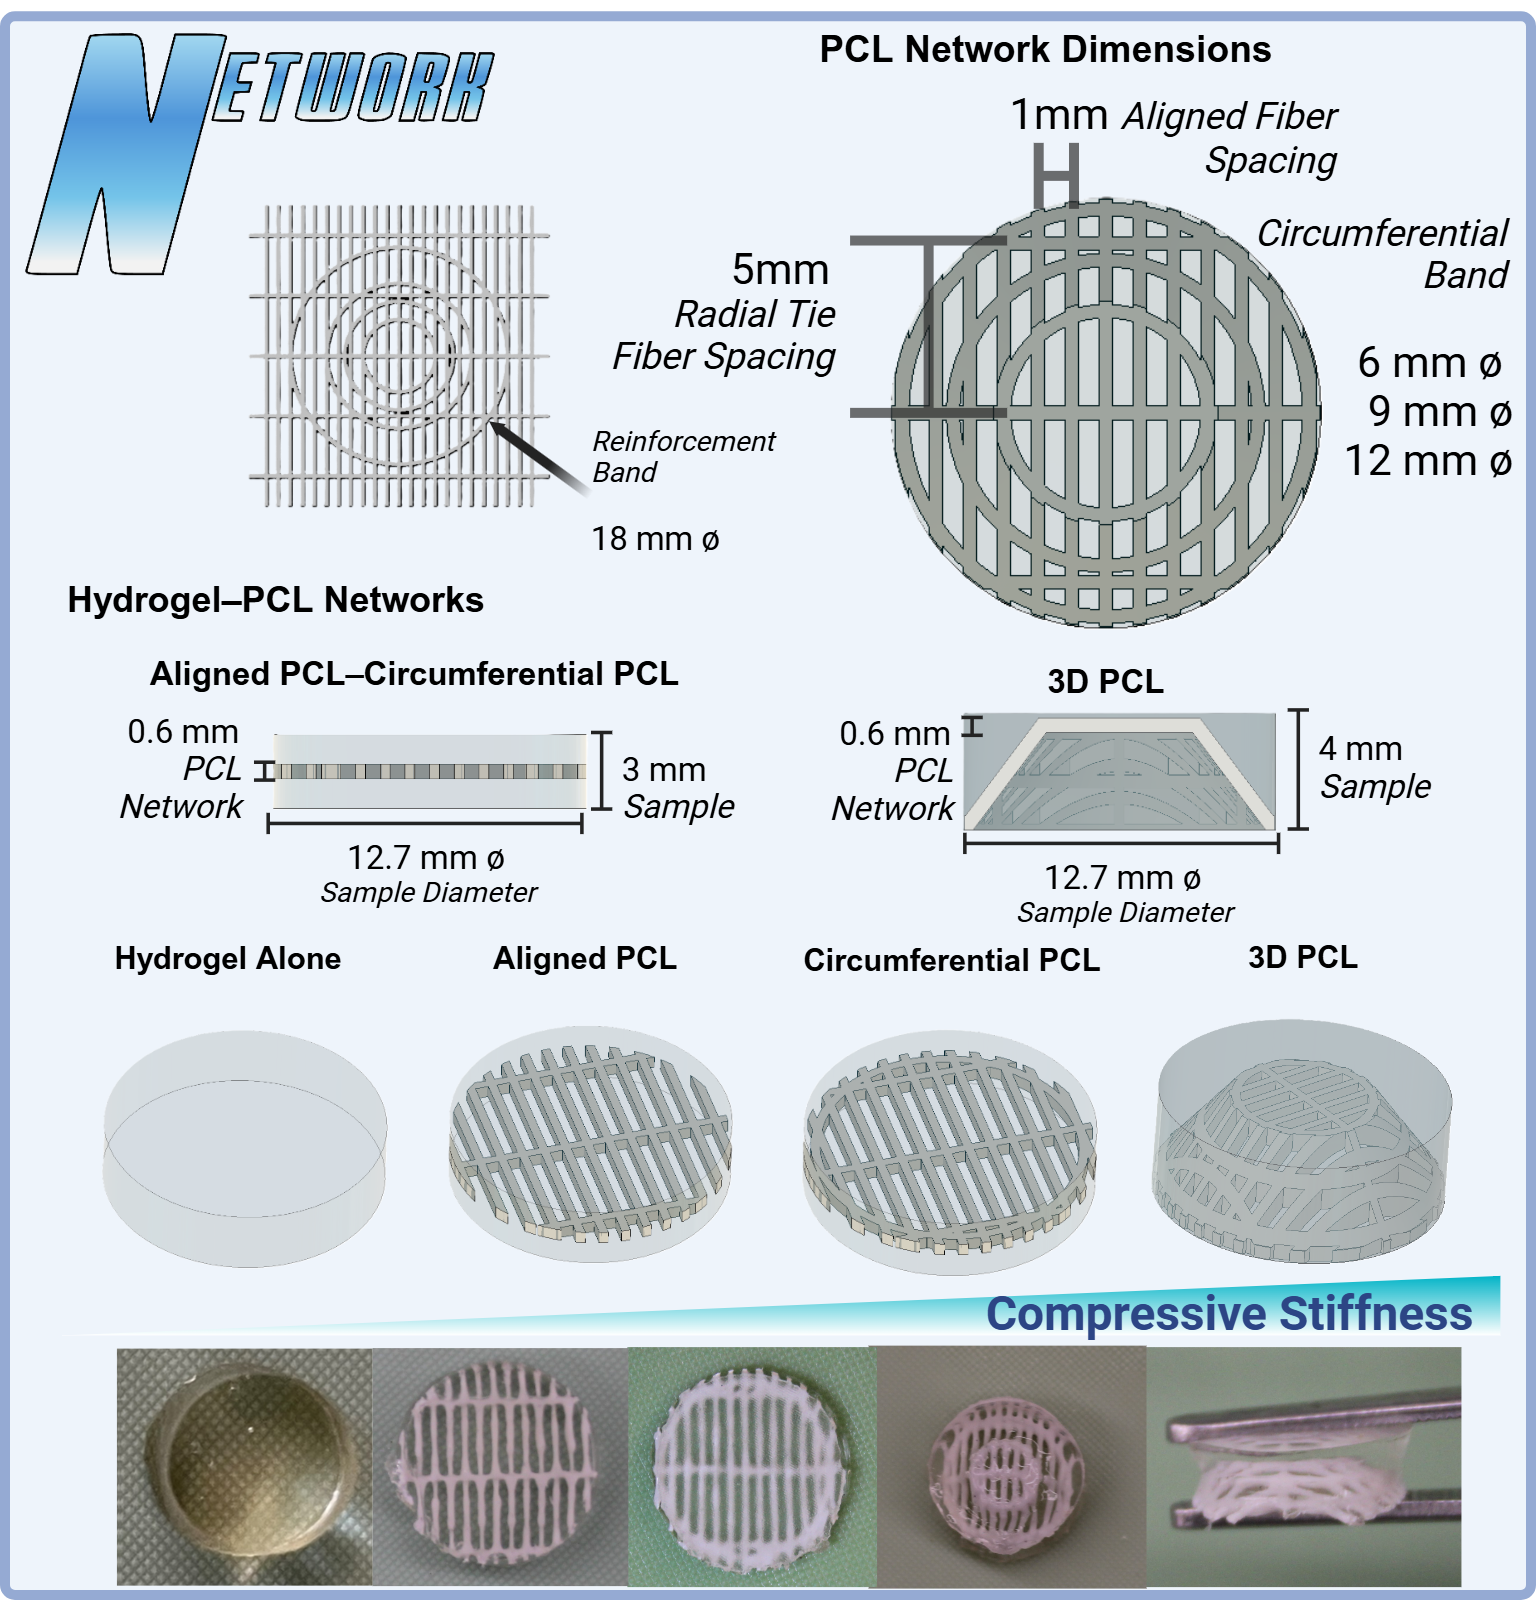
\includegraphics[width=1\linewidth]{figures/chapter 5/ch5_networks.png}
    \caption[PCL Network Designs and Characterization]{\textbf{PCL Network Designs and Characterization.} Schematic representations and cross-sections of PCL network designs showing fiber architectures and dimensional specifications. PCL networks include aligned, circumferential, and 3D thermomolded variants. Bottom panel displays representative samples of each construct group (hydrogel-only control and PCL-reinforced variants) prepared for mechanical characterization.}
    \label{fig:ch5_networks}
\end{figure}

\section{Stress-Relaxation Testing and Analysis}

To characterize the time-dependent mechanical performance of the HANI scaffolds, samples were subjected to a confined compression stress-relaxation protocol. This method enables quantification of viscoelastic behavior, simulating how the scaffold would respond to sustained loading in vivo. 

Each sample was placed in a confined chamber and compressed to a defined strain level. The deformation was held constant while the resulting stress decay was recorded over a specified duration. This allowed for the separation of instantaneous (elastic) response from long-term (viscous) behavior, providing both an initial modulus and an equilibrium stress value for each scaffold type.

The protocol consisted of:
\begin{itemize}
    \item Preload of 0.15 N for 1 minute to establish consistent initial conditions
    \item Stepwise compression to 5\%, 10\%, and 20\% strain
    \item Hold periods of 30 minutes at 5\% and 10\% strain, and 60 minutes at 20\% strain
    \item Continuous force and displacement recording throughout the test
\end{itemize}

By analyzing these parameters across scaffold designs—including hydrogel-only, aligned PCL, circumferential PCL, and 3D thermomolded constructs—comparisons could be drawn regarding their capacity to resist deformation, dissipate load, and recover over time. These findings offer critical insights into scaffold suitability for mimicking native meniscal poroviscoelasticity and guiding future design refinements.

\begin{figure}[H]
    \centering
    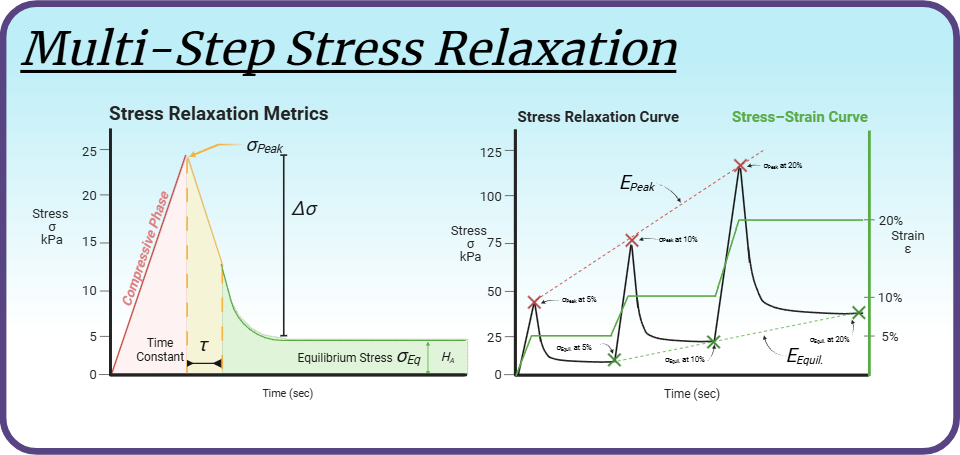
\includegraphics[width=1\linewidth]{figures/chapter 5/ch5_stressRelax.png}
    \caption[Stress-Relaxation Testing Protocol and Apparatus]{\textbf{Stress-Relaxation Testing Protocol and Apparatus.} Schematic representation of confined compression testing setup used to evaluate time-dependent mechanical properties of HANI scaffolds. Samples were subjected to stepwise compression (5\%, 10\%, and 20\% strain) with extended hold periods (30-60 minutes) to characterize stress decay behavior. Key parameters extracted included peak stress ($\sigma_0$), equilibrium stress ($\sigma_{Eq}$), and relaxation time constant ($\tau$).}
    \label{fig:ch5_stressRelax}
\end{figure}

\subsection{Data Analysis Methods}

To further characterize the poroviscoelastic properties, stress relaxation data from each strain level were fitted to a single-phase logarithmic decay model in Python 3.9 using the following stress decay equation:

\begin{equation}
\sigma(t) = \Delta \sigma e^{-t / \tau} + \sigma_{\text{Eq}}
\end{equation}

Where $\sigma_{0}$ represents the peak stress at the start of constant strain hold immediately following compression (t = 0), $\Delta\sigma$ is the initial decay stress equal to the difference between initial peak stress and equilibrium stress, $\tau$ is the relaxation time constant, and $\sigma_{Eq}$ denotes the equilibrium stress measured at the end of each hold phase. The relaxation time constant $\tau$ quantifies how quickly the stress dissipates under constant strain, reflecting the scaffold's ability to redistribute mechanical forces—an essential feature for load-bearing tissues.

\subsection{Mechanical Properties}

To facilitate systematic analysis of the stress-relaxation data, several key mechanical parameters were defined and calculated:

\textbf{Peak Stress ($\sigma_0$):} The maximum stress recorded immediately upon reaching the target strain, representing the scaffold's instantaneous response to compression:
\begin{equation}
\sigma_0 = \frac{F_{\max}}{A}
\end{equation}
where $F_{\max}$ is the maximum force recorded and $A$ is the cross-sectional area of the sample.

\textbf{Equilibrium Stress ($\sigma_{Eq}$):} The stress measured after relaxation has plateaued, indicating the scaffold's capacity for sustained load-bearing:
\begin{equation}
\sigma_{Eq} = \frac{F_{eq}}{A}
\end{equation}
where $F_{eq}$ is the equilibrium force after the hold period.

\textbf{Stress Decay ($\Delta\sigma$):} The difference between peak and equilibrium stress, reflecting the scaffold's viscoelastic behavior:
\begin{equation}
\Delta\sigma = \sigma_0 - \sigma_{Eq}
\end{equation}

\textbf{Time Constant ($\tau$):} A measure of the rate of stress relaxation, derived from fitting the stress-time curve to a single-phase exponential decay model:
\begin{equation}
\sigma(t) = \Delta\sigma \cdot e^{-t/\tau} + \sigma_{Eq}
\end{equation}

\textbf{Peak Modulus ($E_{peak}$):} Quantifies the material's instantaneous stiffness during the initial loading phases. The peak stresses at strain levels ($\varepsilon$ = 5\%, 10\%, 15\%(average) and 20\%) are plotted against the corresponding strains, and the slope of the linear regression line represents the peak modulus:
\begin{equation}
E_{peak} = \frac{\Delta\sigma_{0}}{\Delta\varepsilon}
\end{equation}

The peak modulus reflects the scaffold's resistance to deformation under compressive loads, with a higher slope indicating stiffer hydrogels. The peak modulus is essential for evaluating whether the HANI hydrogels provide the necessary mechanical integrity to handle dynamic joint stresses.

\textbf{Equilibrium Modulus ($E_{Eq}$):} Measures the stiffness of the material at equilibrium, once internal fluid flow has ceased. This modulus is particularly relevant for biological tissues such as cartilage and menisci, where maintaining structural integrity under sustained loads is crucial for long-term functionality. During stress relaxation testing, equilibrium stresses $\sigma_{Eq}$ are recorded at the end of each hold phase:
\begin{equation}
E_{Equil} = \frac{\Delta\sigma_{Eq}}{\Delta\varepsilon}
\end{equation}

\textbf{Aggregate Modulus ($H_A$):} The equilibrium stiffness under confined compression, calculated as:
\begin{equation}
H_A = \frac{\sigma_{Eq}}{\varepsilon}
\end{equation}
where $\varepsilon$ is the applied strain.

\clearpage
\section{Poroviscoelastic Characterization and Mechanical Analysis}

This study introduced a novel method of hydrogel augmentation via the HANI method to mimic the native meniscus by leveraging the poroviscoelastic properties of gelatin-based hydrogels and the structural reinforcement of polycaprolactone (PCL). To achieve physiologically relevant properties, various mass ratios of gelatin to glutaraldehyde (GTA) were evaluated for water content, with the goal of approximating the native meniscus, which exhibits a water content of approximately 76\%. The 100:1 and 300:1 gelatin to GTA mass ratios were selected for further study as they closely matched native meniscal water content but albeit with slightly higher values (Figure 2). This adjustment was intentional, given the plan to incorporate PCL reinforcements, which would increase overall polymer content and modulate water retention.\\[0pt]

Although differences in water content between formulations were not statistically significant, mechanical performance testing revealed substantial variations in load-bearing capacity, compressive stiffness, and stress relaxation behavior. Consequently, the 100:1 and 300:1 gelatin to GTA mass ratios were chosen to further assess the scaffolds' mechanical attributes across various PCL configurations.\\[0pt]

The optimization process further involved integrating PCL reinforcement configurations (aligned, circumferential, and 3D) to enhance anisotropic load distribution, energy dissipation, and structural integrity under dynamic physiological forces. This synergy between chemical and mechanical properties positions the scaffolds as robust candidates for meniscal tissue engineering, demonstrating the potential to withstand repetitive joint loading while maintaining functionality over time \cite{norberg2021viscoelasticequilibrium}.

\begin{figure}[H]
    \centering
    \includegraphics[width=0.87\linewidth]{figures/chapter 5/graphs1.png}
    \caption[Analysis of Peak Stress, Stress Decay, and Equilibrium Stress in HANI Hydrogels]{\textbf{Analysis of Peak Stress, Stress Decay, and Equilibrium Stress in HANI Hydrogels.} Comparison of mechanical properties across different GelA-GTA mass ratios and PCL reinforcement configurations. Statistical significance: *$p < 0.05$, **$p < 0.01$, ***$p < 0.001$, ****$p < 0.0001$.}\label{fig:ch5_stress_analysis}
\end{figure}

\subsection{Peak Stress ($\sigma_0$)}

Peak stress ($\sigma_0$), a measure of the maximum stress a material can sustain under load, exhibited substantial improvements with both increased glutaraldehyde (GTA) concentration and polycaprolactone (PCL) reinforcement (\autoref{fig:ch5_stress_analysis}). For the 300 GTA hydrogels, unreinforced samples displayed modest peak stress values, reaching 2.45 ± 0.20 kPa at a 5\% strain and 9.79 ± 2.47 kPa at a 20\% strain. Aligned PCL reinforcement more than doubled these values, achieving 5.19 ± 1.50 kPa at a 5\% strain and 44.13 ± 13.75 kPa at a 20\% strain. Circumferential PCL reinforcement provided even greater improvements, with $\sigma_0$ reaching 7.25 ± 0.87 kPa at a 5\% strain and 61.90 ± 20.01 kPa at a 20\% strain. Similarly, 3D PCL scaffolds enhanced peak stress to 8.03 ± 1.82 kPa and 49.17 ± 13.17 kPa at 5\% and 20\% strains, respectively.

In the 100 GTA hydrogels, peak stress values were markedly higher than those in the 300 GTA hydrogels for most configurations, except the initial aligned PCL which had slightly lower values at 5\% and 20\% strains, due to the increased cross-linking density. Unreinforced samples exhibited peak stresses of 3.84 ± 0.60 kPa at a 5\% strain and 27.63 ± 4.94 kPa at a 20\% strain. Aligned PCL reinforcement further improved $\sigma_0$, reaching 5.65 ± 1.22 kPa at a 5\% strain and 42.30 ± 11.82 kPa at a 20\% strain. Circumferential PCL reinforcement achieved the highest values, with $\sigma_0$ increasing to 7.54 ± 1.50 kPa at a 5\% strain and 79.38 ± 16.40 kPa at a 20\% strain. The 3D PCL configuration also performed well, with peak stresses reaching 9.04 ± 0.11 kPa at a 5\% strain and 56.16 ± 2.98 kPa at a 20\% strain.

Two-way ANOVA revealed significant effects of strain level and PCL configuration for both GelA--GTA mass ratios on peak stress (p < 0.0001). Post hoc Tukey's tests confirmed that circumferential and 3D PCL configurations significantly outperformed aligned and unreinforced hydrogels (p < 0.05). Among the configurations, circumferential PCL reinforcement in the 100 GTA hydrogels yielded the highest peak stress values, highlighting its superior ability to distribute loads effectively.

These results underscore the importance of the HANI's strategic PCL reinforcement, particularly in the circumferential and 3D configurations, in enhancing the mechanical strength of the hydrogels \cite{boschetti2004biomechanicalproperties,patel2019systematicreview}.

\subsection{Stress Decay ($\Delta\sigma$)}

Stress decay ($\Delta\sigma$), a measure of a material's ability to dissipate stress over time, was significantly influenced by strain level and PCL reinforcement for both GelA--GTA mass ratios (\autoref{fig:ch5_stress_analysis}). At a 300 GTA ratio, unreinforced hydrogels exhibited low stress decay values across all strain levels, with $\Delta\sigma$ reaching only 1.09 ± 0.12 kPa at a 5\% strain and 3.55 ± 1.44 kPa at a 20\% strain. PCL reinforcement improved stress decay significantly, particularly in the circumferential and 3D configurations. Circumferential PCL reinforcement increased $\Delta\sigma$ to 3.18 ± 0.50 kPa at a 5\% strain and 34.59 ± 11.51 kPa at a 20\% strain, nearly ten-fold higher than unreinforced hydrogels. Similarly, the 3D configuration achieved $\Delta\sigma$ values of 3.75 ± 1.11 kPa and 20.23 ± 5.75 kPa at 5\% and 20\% strains, respectively.

In the 100 GTA hydrogels, stress decay values were significantly higher, reflecting the effect of increased cross-linking density. The unreinforced 100 GTA hydrogels demonstrated $\Delta\sigma$ values of 1.92 ± 0.49 kPa at a 5\% strain and 13.66 ± 4.46 kPa at a 20\% strain. With circumferential PCL reinforcement, $\Delta\sigma$ reached 3.16 ± 0.83 kPa at a 5\% strain and 46.03 ± 11.16 kPa at a 20\% strain, the highest value recorded. The 3D PCL configuration also performed well, with $\Delta\sigma$ values of 3.93 ± 0.05 kPa and 21.85 ± 3.32 kPa at 5\% and 20\% strains, respectively.

Two-way ANOVA revealed significant effects of strain level and PCL configuration for both GelA--GTA mass ratios on stress decay (p < 0.0001), with circumferential and 3D PCL reinforcements significantly outperforming aligned and unreinforced hydrogels (p < 0.05). These results indicate that strategic reinforcement, particularly circumferential PCL in a 100 GTA matrix, provides superior stress decay performance \cite{patel2019systematicreview,morejon2020compressiveproperties,norberg2021viscoelasticequilibrium,roberts2011comparativestudy}.

\subsection{Equilibrium Stress ($\sigma_{Eq}$)}

Equilibrium stress ($\sigma_{Eq}$), representing the sustained stress level after initial relaxation, improved significantly for both GelA--GTA mass ratios with strain level and PCL reinforcement (\autoref{fig:ch5_stress_analysis}). For the 300 GTA hydrogels, the unreinforced samples showed low equilibrium stress values, reaching 1.08 ± 0.23 kPa at a 5\% strain and 4.62 ± 0.67 kPa at a 20\% strain. PCL reinforcement markedly improved $\sigma_{Eq}$, particularly in the circumferential and 3D configurations. Circumferential PCL reinforcement increased equilibrium stress to 3.04 ± 0.66 kPa at a 5\% strain and 17.07 ± 5.77 kPa at a 20\% strain, while 3D PCL scaffolds achieved even higher values, reaching 3.34 ± 0.41 kPa and 22.27 ± 7.56 kPa at 5\% and 20\% strains, respectively.

In the 100 GTA hydrogels, $\sigma_{Eq}$ values were significantly higher across all configurations. Unreinforced hydrogels reached 1.52 ± 0.16 kPa at a 5\% strain and 8.21 ± 1.00 kPa at a 20\% strain, while circumferential PCL reinforcement elevated $\sigma_{Eq}$ to 3.45 ± 0.73 kPa at a 5\% strain and 21.78 ± 3.57 kPa at a 20\% strain. The 3D PCL configuration achieved the highest equilibrium stress values in the 100 GTA samples, with $\sigma_{Eq}$ reaching 4.14 ± 0.13 kPa and 25.03 ± 3.83 kPa at 5\% and 20\% strains, respectively.

Statistical analysis confirmed significant effects of both strain level and PCL configuration for both GelA--GTA mass ratios on equilibrium stress (p < 0.0001). Post hoc Tukey's tests indicated that the circumferential and 3D PCL configurations significantly outperformed the aligned and unreinforced hydrogels (p < 0.05), with circumferential PCL yielding the highest sustained stress values overall.

These findings highlight the role of circumferential and 3D PCL reinforcements in enhancing equilibrium stress \cite{boschetti2004biomechanicalproperties,morejon2020compressiveproperties,korhonen2002comparisonequilibrium,norberg2021viscoelasticequilibrium,roberts2011comparativestudy}.

\begin{figure}[H]
    \centering
    \includegraphics[width=0.93\linewidth]{figures/chapter 5/graphs2.png}
    \caption[Analysis of Time Constant and Aggregate Modulus in HANI Hydrogels]{\textbf{Analysis of Time Constant and Aggregate Modulus in HANI Hydrogels.} Bar graphs display time constant ($\tau$) and aggregate modulus ($H_A$) for composite hydrogels with varying GelA-GTA mass ratios (300 and 100) and PCL reinforcement types (no PCL, aligned PCL, circumferential PCL, and 3D PCL) across strain levels of 5\%, 10\%, and 20\%. Statistical significance is denoted by *$p < 0.05$, **$p < 0.01$, ***$p < 0.001$, and ****$p < 0.0001$.}
    \label{fig:ch5_modulus_time_analysis}
\end{figure}


\subsection{Aggregate Modulus ($H_A$)}

The aggregate modulus ($H_A$), representing the compressive stiffness under sustained load, increased significantly with higher strain levels and specific PCL reinforcement configurations for both GelA--GTA mass ratios (\autoref{fig:ch5_modulus_time_analysis}). In the 300 GTA hydrogels, PCL reinforcement---particularly in the circumferential and 3D configurations---markedly improved $H_A$ compared to unreinforced samples, with the 3D configuration achieving the highest values. Similarly, the 100 GTA hydrogels, due to a greater cross-linking density, exhibited consistently higher stiffness across all configurations. The highest $H_A$ values were observed in the 100 GTA hydrogels with 3D PCL reinforcement, indicating superior compressive resistance.

For both GelA--GTA mass ratios, the strain level and PCL reinforcement substantially enhanced the aggregate modulus. Circumferential and 3D PCL reinforcements provided the greatest stiffness improvements, particularly in the 100 GTA hydrogels, where the combination of a high cross-linking density and effective load distribution maximized compressive resistance. These results highlight the potential of these configurations for load-bearing applications like meniscal replacements, where sustained stiffness and structural integrity are crucial.

The increased stiffness in the 100 GTA hydrogels with circumferential and 3D PCL reinforcement closely mirrors the compressive properties of native human meniscal tissue, with aggregate modulus values ranging in the order of 100--150 kPa. These configurations demonstrate the durability and resilience required for long-term orthopaedic applications, making them strong candidates for meniscal tissue engineering. HANI's combination of mechanical robustness and sustained compressive stiffness ensures both immediate load support and enduring performance under cyclic loading conditions \cite{athanasiou2009engineeringknee,boschetti2004biomechanicalproperties,patel2019systematicreview,morejon2020compressiveproperties,morejon2022mechanismsenergy,bahcecioglu20193dprinted}.

\subsection{Time Constant ($\tau$)}

The time constant ($\tau$), indicative of the time required for hydrogels to reach equilibrium stress, exhibited minimal variation across PCL reinforcement types, suggesting limited influence on viscoelastic relaxation properties (\autoref{fig:ch5_modulus_time_analysis}). In the 300 GTA hydrogels, $\tau$ values remained consistent across configurations, with circumferential and 3D PCL reinforcement showing slight decreases compared to unreinforced samples. Similarly, in the 100 GTA hydrogels, $\tau$ values were slightly higher for circumferential and aligned PCL reinforcements but did not show substantial changes \cite{norberg2021viscoelasticequilibrium,disilvestro2001crossvalidationbiphasic}.

The consistent $\tau$ values across strain levels and PCL configurations indicate that PCL reinforcement enhanced mechanical strength without significantly altering the gelatin matrix's intrinsic relaxation dynamics for both GelA--GTA mass ratios. Reinforcement primarily influenced mechanical parameters like peak and equilibrium stress, while preserving viscoelastic stability \cite{norberg2021viscoelasticequilibrium,morejon2020compressiveproperties,patel2019systematicreview}.

The negligible effect of PCL reinforcement on $\tau$ suggests that the hydrogels retained their natural damping properties essential for energy dissipation and shock absorption. These properties, combined with the mechanical benefits of PCL reinforcement, make hydrogels with circumferential and 3D PCL in a 100 GTA matrix particularly suitable for load-bearing applications like meniscal replacements \cite{morejon2022mechanismsenergy,patel2019systematicreview}.

\begin{figure}[H]
    \centering
    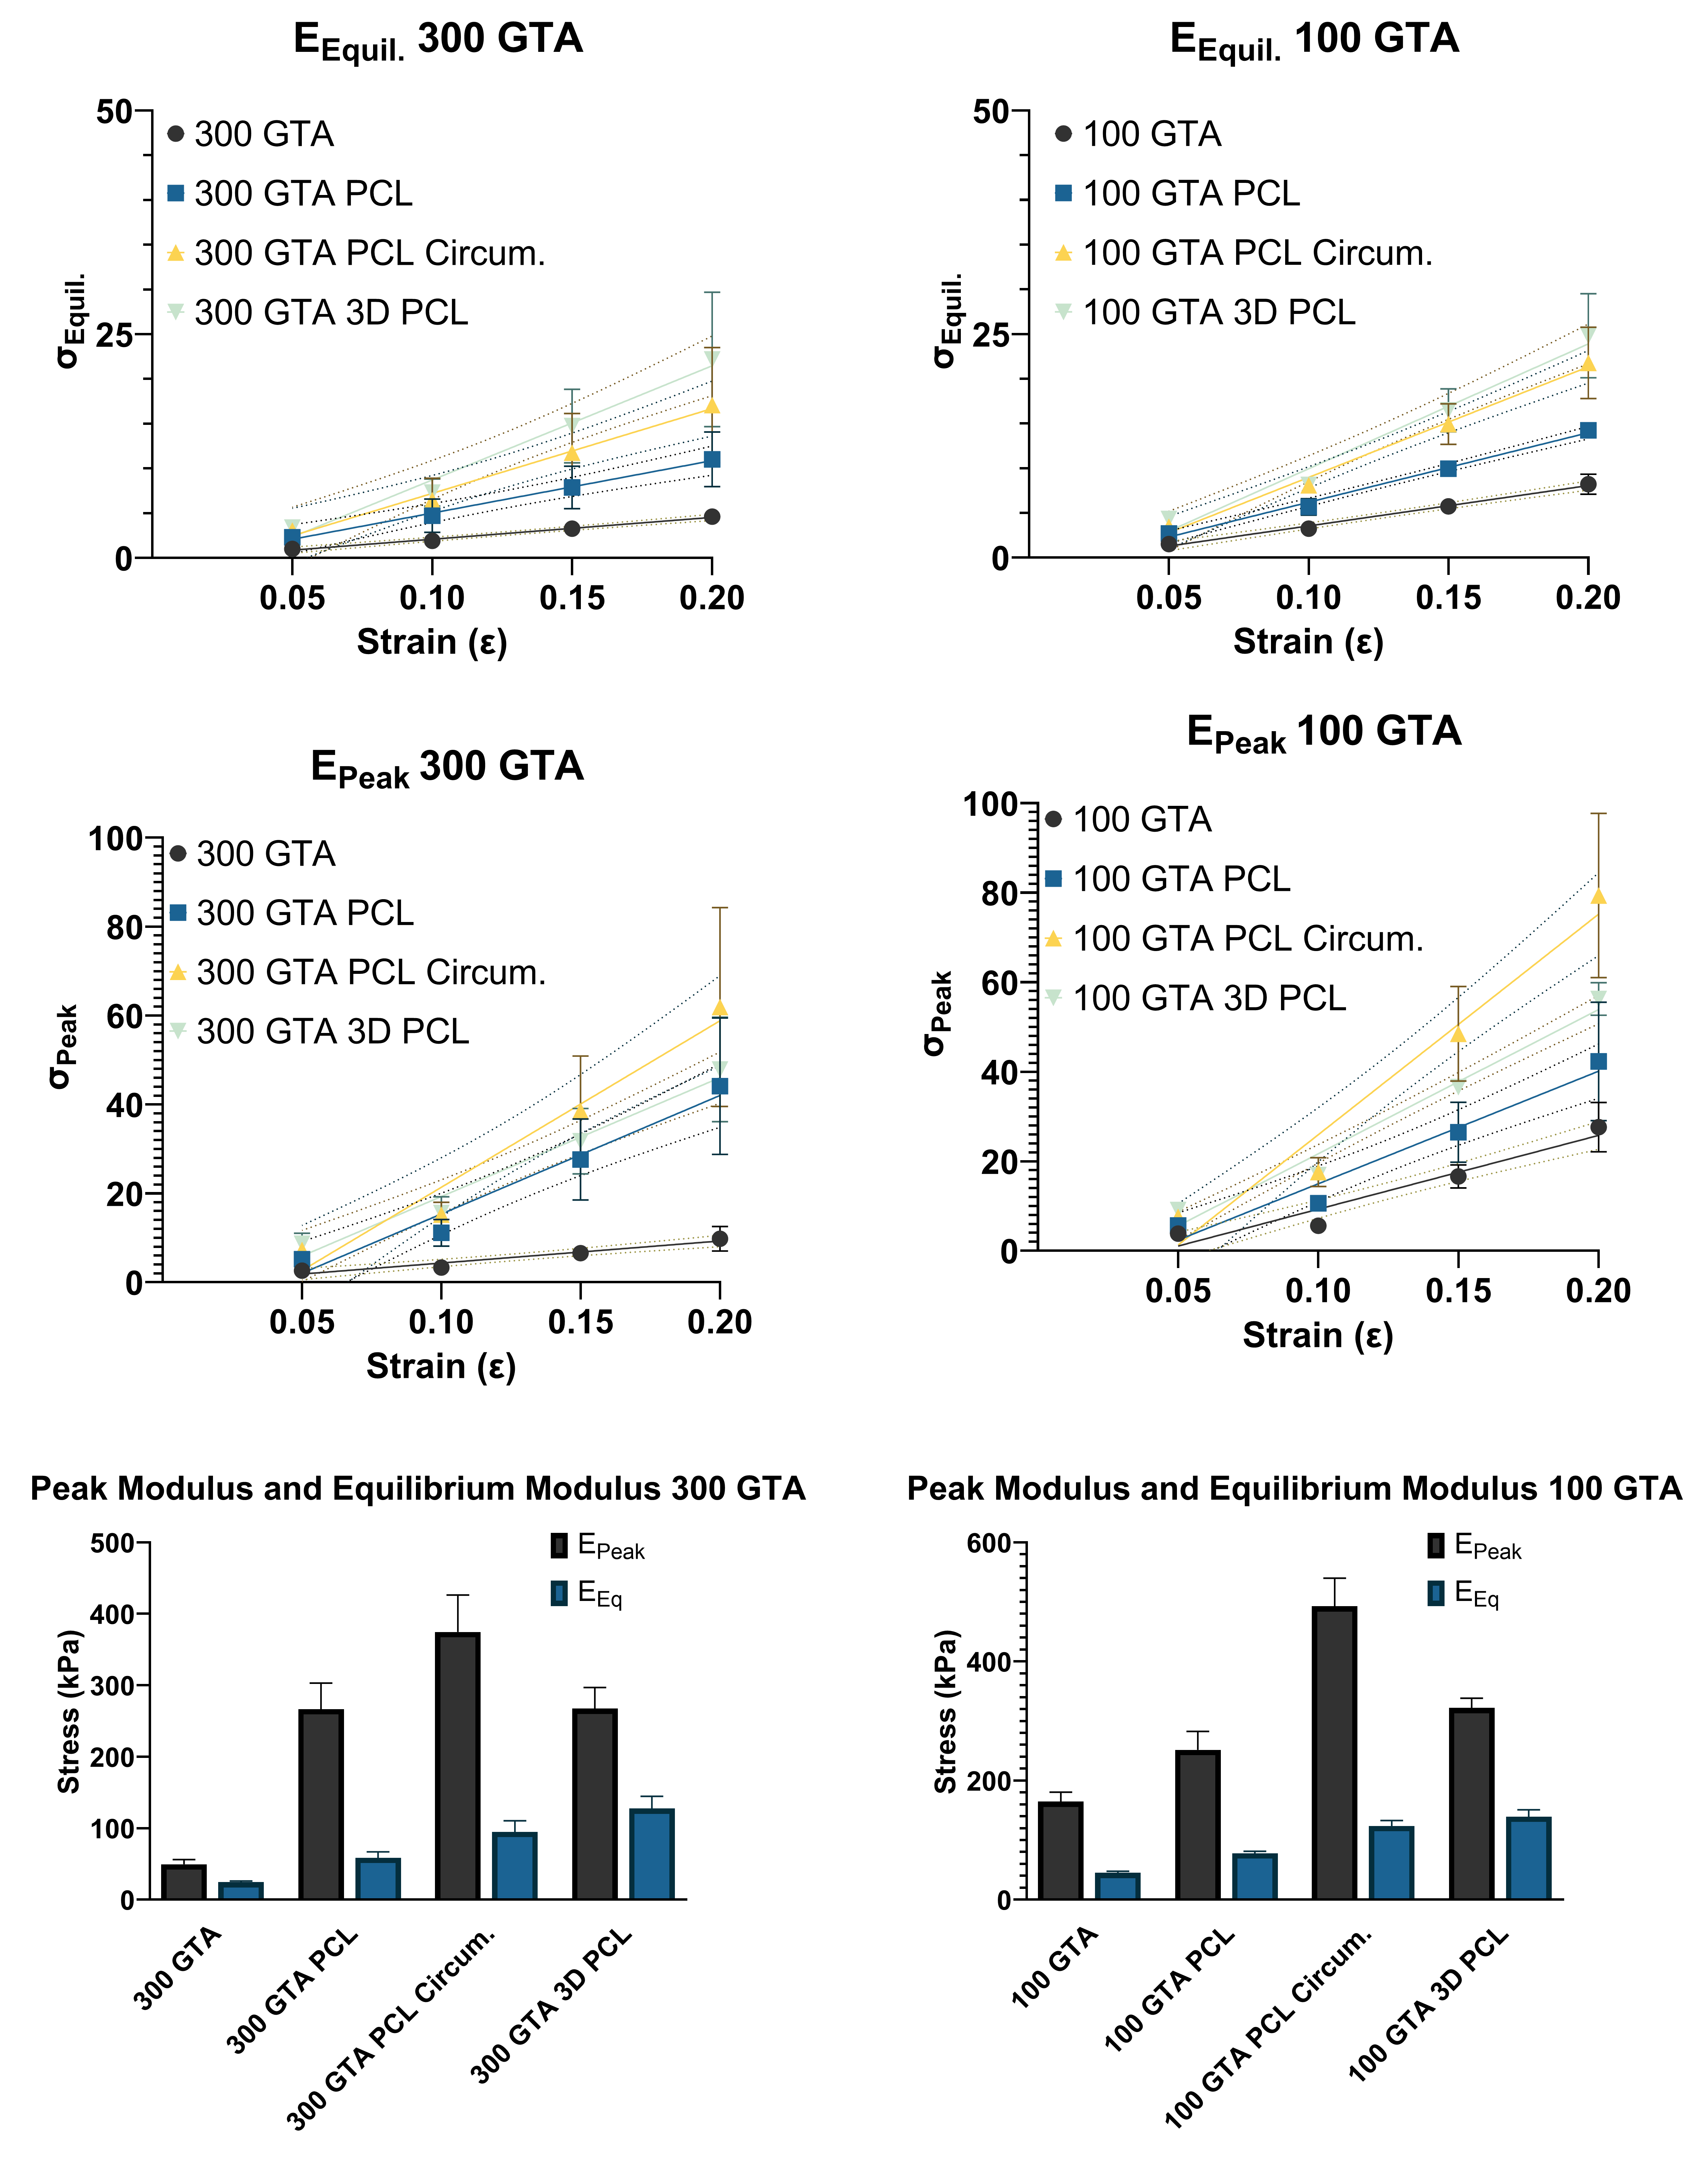
\includegraphics[width=0.9\linewidth]{figures/chapter 5/graphs3.png}
    \caption[Modulus Analysis of HANI Hydrogels]{\textbf{Modulus Analysis of HANI Hydrogels.} Line graphs show peak and equilibrium moduli for HANI hydrogels with 300 and 100 GelA-GTA mass ratios and varying PCL reinforcement types. The slopes correspond to peak modulus ($E_{Peak}$) and equilibrium modulus ($E_{Equil}$). Bar graphs summarize these values across PCL configurations. Error bars represent standard deviations.}
    \label{fig:ch5_modulus_comparison}
\end{figure}

\subsection{Peak Modulus ($E_{peak}$)}

The peak modulus ($E_{peak}$), representing initial stiffness, increased significantly for both GelA--GTA mass ratios across PCL reinforcements (\autoref{fig:ch5_modulus_comparison}). In the 300 GTA hydrogels, unreinforced samples showed a peak modulus of 49.58 kPa, which improved with aligned PCL (266.60 kPa), circumferential PCL (374.60 kPa), and 3D PCL (267.60 kPa). For the 100 GTA hydrogels, the unreinforced modulus of 164.80 kPa increased to 251.60 kPa with aligned PCL and peaked at 492.80 kPa with circumferential PCL. The 3D PCL configuration achieved 322.20 kPa, with a strong model fit (R² = 0.96). Linear regression confirmed significant effects for both GelA--GTA mass ratios across PCL reinforcements on the peak modulus with all configurations having strong model fits (R² > 0.745; p < 0.0001).

The marked improvements in the peak modulus with circumferential and 3D PCL configurations highlight their ability to distribute compressive forces effectively, especially in 100 GTA hydrogels. These enhancements align with the mechanical demands of meniscal tissue engineering, where high initial stiffness is critical for load-bearing applications \cite{bahcecioglu20193dprinted,sun20213dbioprintingreadytoimplant,baek2015meniscustissue}.

\subsection{Equilibrium Modulus ($E_{Equil}$)}

The equilibrium modulus ($E_{Equil}$), indicative of stiffness under sustained loads, showed substantial increases for both GelA--GTA mass ratios with PCL reinforcement (\autoref{fig:ch5_modulus_comparison}). For the 300 GTA hydrogels, the unreinforced modulus of 24.43 kPa rose to 58.59 kPa with aligned PCL, 94.79 kPa with circumferential PCL, and 127.60 kPa with 3D PCL. In the 100 GTA hydrogels, circumferential PCL reached 123.60 kPa, while the highest value, 139.50 kPa, was recorded with 3D PCL.

Linear regression confirmed significant effects for both GelA--GTA mass ratios across PCL reinforcements on the equilibrium modulus with all configurations having strong model fits (R² > 0.735; p < 0.0001) with the exception of the 300 GTA circumferential PCL (R² > 0.672; p < 0.0001).

The high equilibrium modulus values achieved with circumferential and 3D PCL reinforcements in the 100 GTA hydrogels highlight their ability to sustain loads effectively over time. These configurations mirror the sustained stiffness of native meniscal tissue, demonstrating strong potential for use in durable, load-bearing meniscal replacements \cite{a.murphy20243dprintedvariable,bahcecioglu20193dprinted,boschetti2004biomechanicalproperties,patel2019systematicreview}.


\subsection{Design Implications}

HANI's scaffold design leveraged advanced additive manufacturing techniques, combining stereolithography (SLA) and fused deposition modelling (FDM). SLA was pivotal in producing precise molds that preserved alignment and stability of PCL reinforcements, enabling networks to span the scaffold's thickness and mimic the anisotropic properties of the native meniscus \cite{filardo2019patientspecificmeniscus,klarmann20233dprinting,bahcecioglu20193dprinted,ngo2018additivemanufacturing}. FDM enabled continuous fiber printing, creating circumferential and radial-tie fibers that transformed axial compressive loads into tensile stresses. This reinforcement strategy, particularly in the 3D-PCL configuration, ensured progressive load sharing and minimized localized deformation. Together, these techniques produced scaffolds capable of mimicking the hoop stress-strain behavior of the native meniscus, absorbing and redistributing forces effectively to protect surrounding cartilage \cite{filardo2019patientspecificmeniscus,guo20213dprintedcellfree,armiento2018biomaterialsarticular,patel2019systematicreview}.

\subsection{Challenges and Limitations}

It is important to note that variability in PCL placement can occur as a result of molding and fiber misalignment during hydrogel integration; potentially affecting mechanical properties and construct reproducibility. Future developments of the HANI process will focus on optimizing these fabrication techniques to ensure consistent PCL distribution, including the improvement of mold designs and the introduction of thermal stabilization strategies. Additionally, standardizing fabrication protocols and implementing more precise quality control measures, such as real-time imaging during scaffold formation, may help mitigate these inconsistencies in future studies. While the current scaffold fabrication approach produces reinforced hydrogel constructs with improved short-term mechanical performance, long term degradation and in vivo stability remain unexplored. Future research will focus on assessing scaffold behavior under physiological conditions in both in vitro and in vivo settings. These studies will be essential to validate the scaffold's durability and clinical applicability for meniscal tissue engineering.

\section{Summary of HANI Platform Development}

In this study, a novel scaffold fabrication strategy---Hybrid Hydrogels Augmented via Additive Network Integration (HANI)---was developed to address the critical mechanical and biological challenges in meniscal tissue engineering~\cite{makris2011kneemeniscus, gupta2020meniscaltissue}. By integrating architecturally controlled polycaprolactone (PCL) networks within gelatin-based hydrogels, the HANI method successfully enhanced scaffold mechanical performance while preserving the poroviscoelastic behavior essential for mimicking native meniscal tissue~\cite{bulle2021humanmeniscus}.

Specifically, scaffolds reinforced with circumferential and three-dimensional (3D) PCL configurations exhibited substantial increases in peak stress, equilibrium stress, and aggregate modulus compared to hydrogel-only controls. Importantly, the intrinsic viscoelastic relaxation properties of the gelatin phase remained largely unaltered, indicating that mechanical reinforcement did not compromise time-dependent fluid flow behavior critical for joint function~\cite{abdelgaied2015comparisonbiomechanical}.

These findings demonstrate that the strategic integration of multi-directional PCL fibers can recapitulate the anisotropic load-bearing mechanisms of the native meniscus~\cite{elkommos2025hybridhydrogels}. Moreover, the use of additive manufacturing techniques such as stereolithography (SLA) and fused deposition modeling (FDM) allowed for precise spatial control over reinforcement architectures, paving the way for customizable, patient-specific implant fabrication~\cite{filardo2019patientspecificmeniscus}.

\subsection{Primary Technical Achievement}

The primary technical achievement of this work represents the first demonstration of a hybrid scaffold platform combining tunable gelatin hydrogels with thermoformed, 3D PCL reinforcement networks~\cite{elkommos2025hybridhydrogels}. This innovative approach successfully integrates the poroviscoelastic properties of gelatin-based hydrogels with the structural reinforcement capabilities of polycaprolactone, creating a composite material that mimics the mechanical behavior of native meniscal tissue~\cite{bulle2021humanmeniscus, abdelgaied2015comparisonbiomechanical}. The HANI methodology enables precise control over both the hydrogel matrix composition and the spatial distribution of PCL reinforcement, allowing for tailored mechanical properties that can be optimized for specific clinical applications~\cite{gupta2020meniscaltissue}.

\subsection{Performance Highlights}

The HANI platform demonstrated enhanced compressive mechanical properties while maintaining stress-relaxation behavior characteristic of native meniscus~\cite{bulle2021humanmeniscus}. Specifically, circumferential and 3D PCL configurations achieved peak stress values up to 79.38 ± 16.40 kPa and equilibrium stresses of 139.50 kPa, representing substantial improvements over hydrogel-only controls. These configurations also exhibited superior aggregate modulus values (100--150 kPa) that closely match native meniscal tissue properties~\cite{abdelgaied2015comparisonbiomechanical}. Importantly, the time constant ($\tau$) remained consistent across all reinforcement configurations, indicating that mechanical enhancement did not compromise the essential viscoelastic relaxation dynamics required for proper joint function~\cite{makris2011kneemeniscus}.

\subsection{Clinical and Research Implications}

The modularity and scalability of the HANI platform align closely with the future of personalized orthopaedic repair strategies, offering a blueprint for next-generation meniscal replacements~\cite{filardo2019patientspecificmeniscus, gupta2020meniscaltissue}. The ability to customize both hydrogel composition and PCL architecture enables patient-specific implant design based on individual biomechanical requirements and anatomical considerations~\cite{makris2011kneemeniscus}. Furthermore, the use of additive manufacturing techniques facilitates reproducible fabrication of complex reinforcement patterns, supporting clinical translation and regulatory approval processes~\cite{elkommos2025hybridhydrogels}. This platform establishes a foundation for developing load-responsive, durable meniscal implants that can withstand the demanding mechanical environment of the knee joint while promoting tissue integration and long-term functionality~\cite{bulle2021humanmeniscus}.

The modularity and scalability of the HANI platform align closely with the future of personalized orthopaedic repair strategies, offering a blueprint for next-generation meniscal replacements~\cite{filardo2019patientspecificmeniscus, gupta2020meniscaltissue}. The ability to customize both hydrogel composition and PCL architecture enables patient-specific implant design based on individual biomechanical requirements and anatomical considerations~\cite{makris2011kneemeniscus}. Furthermore, the use of additive manufacturing techniques facilitates reproducible fabrication of complex reinforcement patterns, supporting clinical translation and regulatory approval processes~\cite{elkommos2025hybridhydrogels}. This platform establishes a foundation for developing load-responsive, durable meniscal implants that can withstand the demanding mechanical environment of the knee joint while promoting tissue integration and long-term functionality~\cite{bulle2021humanmeniscus}.





















































































































































































































































































































































































































































































































































































































































































































































































































































































































































































































































































































































































































































































































































































































































































































































































































































































































































































































































































































































































































































































































































































































































































































































































































































































































































































































































































































































































































































































































































































































































































































































































































































































































































































































































































































































































































































































































































































































































































































































































































































































































































































































































































































































































































































































































































































































































































































































































































































































































































































































































































































































































































































































































































































































































































































































































































































































































































































































































































































































































































































































































































































































































































































































































































































































































































































































































































































































































































































































































































































































































































































































































































































































































































































































































































































































































































































































































































































































































































































































































































































































































































































































































































































































































































































































































































































































































































































































































































































































































































































































































































































































































































































































































































































































































































































































































































































































































































































































































































































































































































































































































































































































































































































































































































































































































































































































































































































































































































































































































































































































































































































































































































































































































































































































































































































































































































































































































































































































































































































































































































































































































































































































































































































































































































































































































































































































































































































































































































































































































































































































































































































































































































































































































































































































































































































































































































































































































































































































































































































































































































































































































































































































































































































































































































































































































































































































































































































































































































































































































































































































































































































































































































































































































































































































































































































































































































































































































































































































































































































































































































































































































































































































































































































































































































































































































































































































































































































































































































































































































































































































































































































































































































































































































































































































































































































































































































































































































































































































































































































































































































































































































































































































































































































































































































































































































































































































































































































































































































































































































































































































































































































































































































































































































































































































































































































































































































































































































































































































































































































































































































































































































































































































































































































































































































































































































































































































































































































































































































































































































































































































































































































































































































































































































































































































































































































































































































































































































































































































































































































































































































































































































































































































































































































































































































































































































































































































































































































































































































































































































































































































































































































































































































































































































































































































































































































































































































































































































































































































































































































































































































































































































































































































































































































































































































































































































































































































































































































































































































































































































































































































































































































































































































































































































































































































































































































































































































































































































































































































































































































































































































































































































































































































































































































































































































































































































































































































































































































































































































































































































































































































































































































































































































































































































































































































































































































































































































































































































































































































































































































































































































































































































































































































































































































































































































































































































































































































































































































































































































































































































































































































































































































































































































































































































































































































































































































































































































































































































































































































































































































































































































































































































































































































































































































































































































































































































































































































































































































































































































































































































































































































































































































































































































































































































































































































































































































































































































































































































































































































































































































































































































































































































































































































































































































































































































































































































































































































































































































































































































































































































































































































































































































































































































































































































































































































































































































































































































































































































































































































































































































































































































































































































































































































































































































































































































































































































































































































































































































































































































































































































































































































































































































































































































































































































































































































































































































































































































































































































































































































































































































































































































































































































































































































































































































































































































































































































































































































































































































































































































































































































































































































































































































































































































































































































































































































































































































































































































































































































































































































































































































































































































































































































































































































































































































































































































































































































































































































































































































































































































































































































































































































































































































































































































































































































































































































































































































































































































































































































































































































































































































































































































































































































































































































































































































































































































































































































































































































































































































































































































































































































































































































































































































































































































































































































































































































































































































































































































































































































































































































































































































































































































































































































































































































































































































































































































































































































































































































































































































































































































































































































































































































































































































































































































































































































































































































































































































































































































































































































































































































































































































































































































































































































































































































































































































































































































































































































































































































































































































































































































































































































































































































































































































































































































































































































































































































































































































































































































































































































































































































































































































































































































































































































































































































































































































































































































































































































































































































































































































































































































































































































































































































































































































































































































































































































































































































































































































































































































































































